\documentclass[11pt,letterpaper]{article}
\usepackage[utf8]{inputenc}
\usepackage{amsmath,amssymb,fullpage,graphicx}
\usepackage{subfigure}
\let\hat\widehat
\let\tilde\widetilde

\begin{document}
\subsection*{Q1-a}
\noindent $R = (\frac{X_1 - \bar{X}}{\sigma \sqrt{1 - \frac{1}{n}}}, \frac{X_2 - \bar{X}}{\sigma \sqrt{1 - \frac{1}{n}}}...\frac{X_n - \bar{X}}{\sigma \sqrt{1 - \frac{1}{n}}})$ where $\bar{X}$ denotes sample mean, $S$ denotes sample standard deviation. 

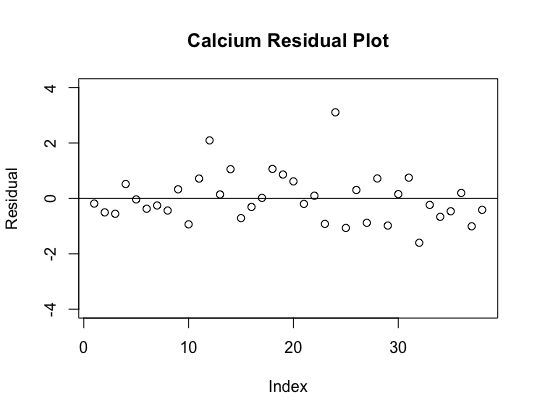
\includegraphics[scale=0.6]{q1-a.png}

\noindent Most residuals fall in -2 to 2, which implies most data is included in 2 standard deviations from mean value. Residuals are denser when close to zero than away from zero. Though there is one extreme value that lies outside 3rd standard deviations away from the mean, the dataset seems to follow normal distribution.\\

\noindent (R code in Appendix)

\subsection*{Q1-b}
\noindent $Y-axis = R$ where $R$ is the standardized residual for calcium value. 
\begin{align*}
F_R(r) &= P(R \leq r) \\
&= P(\frac{X - \bar{X}}{\sigma \sqrt{1 - \frac{1}{n}}} \leq r) 
\end{align*}
\noindent Since $X$ is hypothesized to follow normal distribution, $\frac{X - \bar{X}}{\sigma \sqrt{1 - \frac{1}{n}}} = Z$, $F(r) = P(Z \leq r) = \Phi(r)$
\begin{align*}
Y-axis \text{ vs } X-axis &= \Phi(r_k) \text{ vs } \frac{k}{n+1} \\
&= r_k \text{ vs } \Phi^{-1}(\frac{k}{n + 1})
\end{align*}
\includegraphics[scale=0.6]{Q1-b.png}

\noindent From the QQ-plot, we can perceive that residuals in the middle match with expected values very well. However, a few data points on two tails is larger than expected value, since the density of standardized residual is lower in left tail and higher in right tail than of standard normal. Overall, the distribution of standardized residuals follows normal distribution. 

\subsection*{Q1-c}
\noindent Since we presume the population variance $\sigma $ is known, the ancillary statistic $R$ is defined as $(X_1 - \bar{X}, X_2 - \bar{X}...X_n - \bar{X})$. \\

\noindent Use $D(x) = \frac{1}{\sigma^2} \sum_{i=1}^{n}R_i^2$ as discrepancy statistic. \\

\noindent Under normality model, the discrepancy statistic follows chi-square distribution with degree of freedom $n-1$ where n is sample size. In this case $D(x) \sim \chi^{2}_{37}$.

\noindent The observed discrepancy is $29.45$ with its p-value of $0.806825$. Under the test size $\sigma = 0.05$, the observed data failed to provide significant evidence to reject normal model. \\

\noindent (R code in Appendix)

\subsection*{Q1-d}
\noindent Let $p_1, p_2, p_3, p_4$ denote multinomial probabilities for each interval based on presumed model. $\sigma = 500$ and $\theta$ is unknown
\begin{align*}
p_1 &= \int_{-\infty}^{600} \frac{1}{\sqrt{2 \pi \sigma^2}} e^{- \frac{(x-\theta)^2}{2 \sigma^2}} dx \\
&= \Phi (\frac{600 - \theta}{500}) \text{, where } \Phi \text{ is cdf of standard normal} \\
p_2 &= \Phi (\frac{1200 - \theta}{500}) - \Phi (\frac{600 - \theta}{\sigma}) \\
p_3 &= \Phi (\frac{1800 - \theta}{500}) - \Phi (\frac{1200 - \theta}{\sigma}) \\
p_4 &= 1 - \Phi (\frac{1800 - \theta}{500}) \\
\end{align*}
\noindent Let $x_1, x_2, x_3, x_4$ denote number of observed data that fall in each interval. \\

\noindent $x_1 = 9, x_2=20, x_3=7, x_4=2$

\noindent Then the likelihood function based on observed data and presumed multinomial probability can be represented as 
\begin{align*}
L(\theta | x_1, x_2, x_3, x_4) &= \frac{n!}{\prod_{i=1}^{4} (x_i)} \prod_{i=1}^{4} (p_i)^{x_i}\\
&\propto \prod (p_i)^{x_i} \\
&\propto \Phi (\frac{600 - \theta}{\sigma})^9 \times [\Phi (\frac{1200 - \theta}{\sigma}) - \Phi (\frac{600 - \theta}{\sigma})]^{20} \\
& \times [\Phi (\frac{1800 - \theta}{\sigma}) - \Phi (\frac{1200 - \theta}{\sigma})]^{7} \times [1 - \Phi (\frac{1800 - \theta}{\sigma})]^{2}
\end{align*}

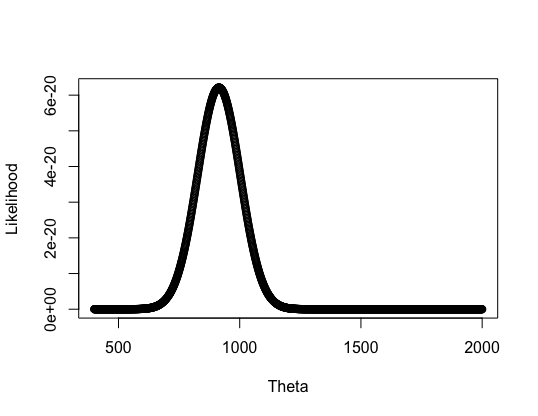
\includegraphics[scale=0.5]{q1-d}

\noindent Based on calculation, the MLE of $\theta$ is equal to $914.2893 $, with initial value 1000 \\

\noindent Based on MLE, values in each interval are 10.122625 17.152466  9.286662  1.438248\\

\noindent The discrepancy statistic is calculated as 
\begin{align*}
D(x) &= \sum_{i=1}^{4} \frac{(x_i - np_i)^2}{np_i} \\
&= 1.379686
\end{align*}
\noindent There are four categories and one unknown parameter, thus, degree of freedom is 2.
\begin{align*}
p-value &= P(\chi^2_2 \geq D(x)) \\
&= 0.5016549
\end{align*}

\noindent chi-square test p-value of observed data is 0.5016549, therefore, under test size 0.05, observed data failed to provide significant evidence that normality model is incorrect.\\

\noindent (R code in Appendix)



\end{document}